\begin{mainquestion}{capacitornetwork}{DC Capacitor Network}

Consider a network of ten capacitors arranged between two nodes A and B as shown below.

\begin{center}
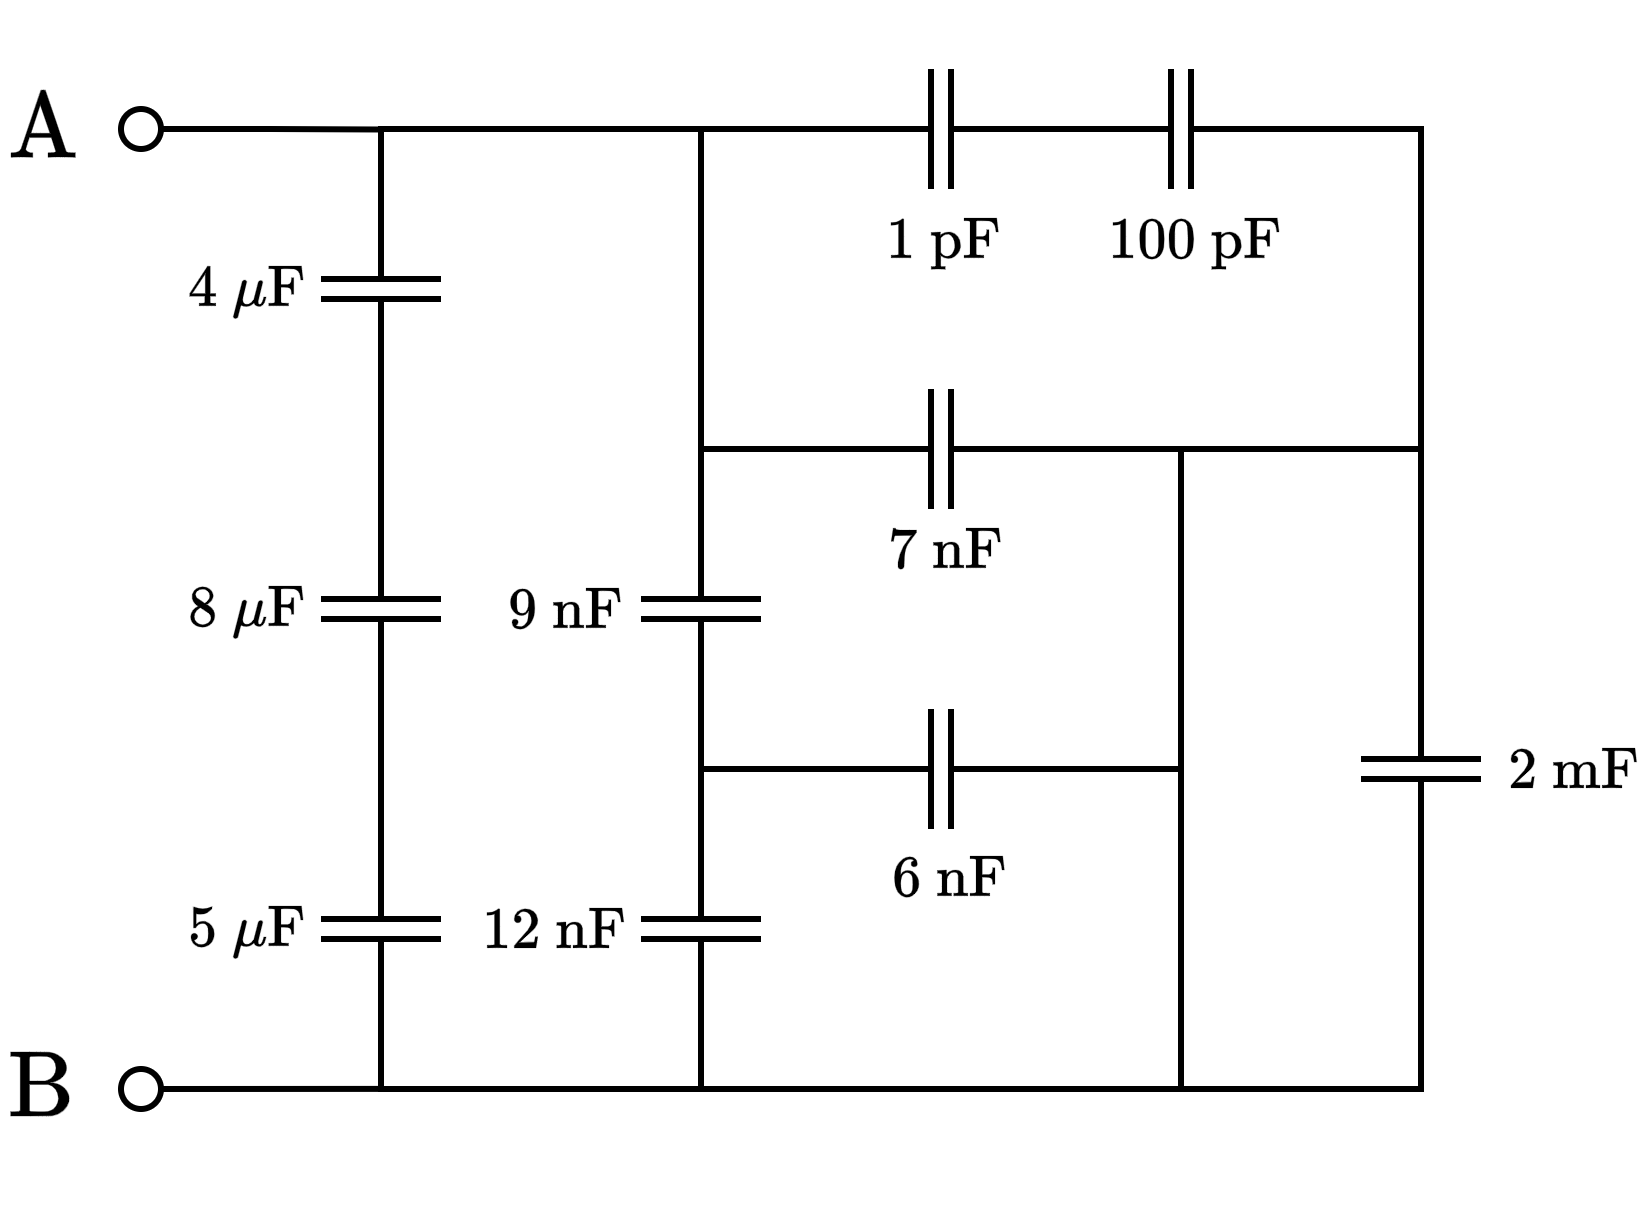
\includegraphics[width=0.8\textwidth]{questionbank/circuit_quantities/capacitor_network/v1/network_diagram.png}
\end{center}

% =========================================================
\begin{partquestion}{networksteadycurrent}
{Calculate the steady-state current through each capacitor if a \qty{12}{\volt} battery is placed between A and B.}

\begin{answer}
At steady state, each capacitor will act like an open circuit and there will be no current through any of the capacitors. Therefore, all capacitor currents are zero.
\end{answer}
\end{partquestion}

% =========================================================
\begin{partquestion}{networksteadyvoltage}
{Calculate the voltage across each capacitor if a \qty{12}{\volt} battery is placed between A and B. Label the capacitor network with the voltages you found. Assume the higher potential is connected to node A.}

\begin{answer}
The voltage is a little more complicated, but there are still some easy ones. Notice how the 7nF capacitor is connected directly to both A and B. This means it's in parallel with the battery so its voltage
\[V_{C7} = \qty{12}{\volt}\]
The next easy one is our 2mF capacitor out on the right. Notice that both of its terminals are connected to B. Since an ideal wire connects both sides of the capacitor, it's not possible for it to hold any voltage, it has been 'shorted out', so its voltage \[V_{C2} = \qty{0}{\volt}\]
Next let's attack the 1pF and 100pF capacitors up near the top. KVL lets us recognize that the sum of their voltages should add up to the battery voltage
\[V_{C1} + V_{C100} = \qty{12}{\volt}\]
Additionally, they also share current since they are in series. Since the current is the rate of change of charge, this also implies they store the same total charge $Q_{C1} = Q_{C100}$ (assuming no charge was stored before we started). Using the definition of charge on a capacitor we can write
\[C_1V_{C1}=C_{100}V_{C100}\]
Combining with the previous equation:
\begin{align*}
V_{C1} + \frac{C_{1}}{C_{100}}V_{C1} &= 12 \\
V_{C1} &= \frac{12C_{100}}{C_1 + C_{100}} \\
V_{C1} &= \frac{\qty{12}{\volt}\cdot\qty{100}{\pico\farad}}{\qty{1}{\pico\farad} + \qty{100}{\pico\farad}} = \frac{\qty{1200}{\volt\pico\farad}}{\qty{101}{\pico\farad}} \approx 11.9\text{ V} \\
V_{C100} &= 12 - V_{C1} \\
V_{C100} &\approx 12 - 11.9 = \qty{0.1}{\volt}
\end{align*}
Interesting, notice that most of the voltage is on the smaller capacitor. That's the reverse of what we see in a resistive voltage divider, where the larger resistor has most of the voltage across it. Also take note that the units of \unit{\pico\farad} canceled out. More generally, this shows that it's the ratio of the capacitance values that matters here, not the magnitude of the capacitance. Hence in future calculations we can neglect the units if they are all the same.

Let's take the string of three capacitors on the right, now that we know how to handle capacitors in series. As before we can write $Q_{C4} = Q_{C8} = Q_{C5} = Q_{string}$ and $V_{C4} + V_{C8} + V_{C5} = 12$. This time, let's set up the equation a little differently by recognizing that $V = Q/C$. This lets us write the following:
\begin{align*}
\frac{Q_{C4}}{C_4} + \frac{Q_{C8}}{C_8} + \frac{Q_{C5}}{C_5} &= 12 \\
Q_{string}(\frac{1}{C_4} + \frac{1}{C_8} + \frac{1}{C_5}) &= 12 \\
Q_{string} &= \frac{12}{(\frac{1}{C_4} + \frac{1}{C_8} + \frac{1}{C_5})} \\
Q_{string} &= \frac{12}{(\frac{1}{\qty{4}{\micro\farad}} + \frac{1}{\qty{8}{\micro\farad}} + \frac{1}{\qty{5}{\micro\farad}})} \\
Q_{string} &= \qty{12}{\volt} \cdot \frac{40}{23}\unit{\micro\farad} = \frac{480}{23}\unit{\micro\coulomb}
\end{align*}

Now that we have $Q_{string}$ we can solve for each capacitor voltage directly using $V = Q/C$.
\begin{align*}
    V_{C4} &= \frac{Q_{string}}{C_4} = \frac{\frac{480}{23}\unit{\micro\coulomb}}{\qty{4}{\micro\farad}} = \frac{120}{23} \approx \qty{5.22}{\volt} \\
    V_{C8} &= \frac{Q_{string}}{C_8} = \frac{\frac{480}{23}\unit{\micro\coulomb}}{\qty{8}{\micro\farad}} = \frac{60}{23} \approx \qty{2.61}{\volt} \\
    V_{C5} &= \frac{Q_{string}}{C_5} = \frac{\frac{480}{23}\unit{\micro\coulomb}}{\qty{5}{\micro\farad}} = \frac{96}{23} \approx \qty{4.17}{\volt}
\end{align*}
As a sanity check, we can show that $5.22 + 2.61 + 4.17 = 12$. Notice again how the largest voltage is across the smallest capacitor.

The last remaining voltages to be found are for the 9nF, 6nF and 12nF capacitors in the middle. This looks more complicated since this isn't a simple series string of capacitors. However, we can use parallel combinations to simplify the problem. Since the 12nF and 6nF capacitors are in parallel, they will share the same voltage! That means we can combine them into one capacitor without losing access to the variables we care about. Capacitors simply add in parallel $\qty{12}{\nano\farad} + \qty{6}{\nano\farad} = \qty{18}{\nano\farad}$, so we will place an effective 18nF cap in the place of the 6nF and 12nF. Now we have the same situation as before, with $C_9$ in series with $C_{18}$.

\begin{align*}
V_{C9} + \frac{C_{9}}{C_{18}}V_{C9} &= 12 \\
V_{C9} &= \frac{12C_{18}}{C_9 + C_{18}} \\
V_{C9} &= \frac{12 \cdot 18}{9 + 18} = \frac{216}{27} = \qty{8}{\volt} \\
V_{C18} &= 12 - V_{C9} \\
V_{C18} &= 12 - 8 = \qty{4}{\volt} \\
\end{align*}

Recalling that the voltage across our $C_{18}$ combo will be the same as it's original parts, we have
\[V_{C6} = V_{C12} = \qty{4}{\volt}\]

We can now summarize our results for our own tidiness and then relabel the original schematic as required. Since the higher potential is at node A, we label each capacitor with the positive end towards node A since that must have been where the charging current originated from.

\begin{table} [h]
    \centering
    \begin{tabular}{| c | c |}
        \hline
        Capacitor & Voltage \\ \hline
        $C_{1}$ & 11.9 \\
        $C_{2}$ & 0 \\
        $C_{4}$ & 5.22 \\
        $C_{5}$ & 4.17 \\
        $C_{6}$ & 4 \\
        $C_{8}$ & 2.61 \\
        $C_{7}$ & 12 \\
        $C_{9}$ & 8 \\
        $C_{12}$ & 4 \\
        $C_{100}$ & 0.1 \\
        \hline
    \end{tabular}
\end{table}

\begin{center}
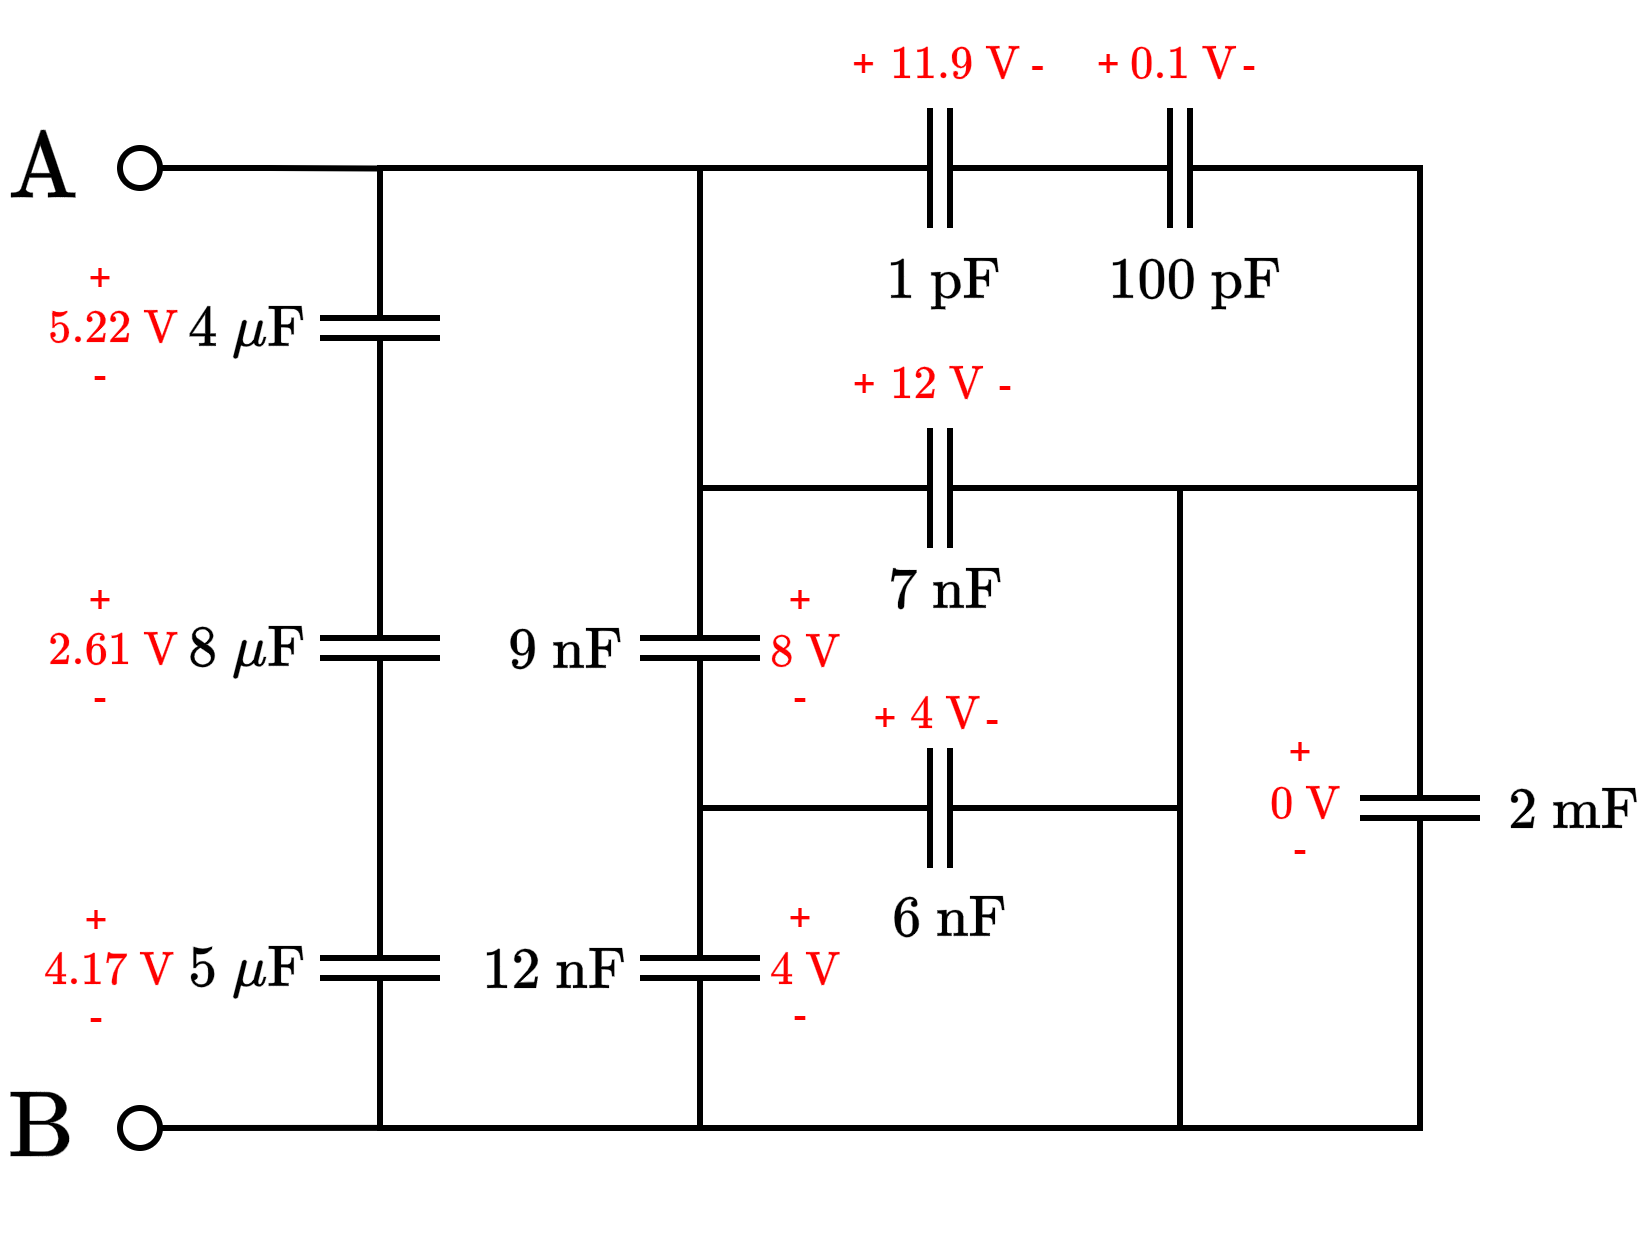
\includegraphics[width=0.8\textwidth]{questionbank/circuit_quantities/capacitor_network/v1/network_diagram_sol.png}
\end{center}

\end{answer}
\end{partquestion}

\begin{partquestion}{energy}
{Which capacitor stores the most energy in part (\cref{prob:capacitornetwork:networksteadyvoltage})?}

\begin{answer}
    The energy in a capacitor is $E_C = \frac{1}{2}CV^2$. Since energy scales with capacitance, let's check the largest capacitors first. The \qty{2}{\milli\farad} cap will not store any energy since it has \qty{0}{\volt} across it. Let's compare the energy stored in the \unit{\micro\farad} capacitors.

    \begin{table} [h]
    \centering
    \begin{tabular}{| c | c | c |}
        \hline
        Capacitor & Voltage (V) & Energy (\unit{\micro\joule)} \\ \hline
        \textcolor{red}{$C_{4}$} & \textcolor{red}{5.22} & \textcolor{red}{54.5}\\
        $C_{5}$ & 4.17 & 43.5\\
        $C_{8}$ & 2.61 & 27.2\\
        \hline
    \end{tabular}
\end{table}

Looks like $C_4$ stores the most energy. We don't need to consider any of the other capacitors since they are all at least $\times1000$ smaller. Even if they were charged to the maximum battery voltage, that would only scale up the energy by $12^2 = \times144$. This guarantees they are smaller.

    
\end{answer}
\end{partquestion}

\end{mainquestion}
